% Created by Christoph Jansen
% License: CC BY 4.0 http://creativecommons.org/licenses/by/4.0/
% Source: https://github.com/Gnork/htw-latex-template
% THIS TEMPLATE IS NOT OFFICIAL
% Offical .doc template: http://www.htw-berlin.de/hochschulstruktur/zentrale-referate/presse-und-oeffentlichkeitsarbeit/abschlussarbeiten-vorlagen/

\documentclass[a4paper]{book}
\usepackage[twoside=false,margin=2.5cm,bindingoffset=2cm]{geometry}
%% select english for this paper
\usepackage[english]{babel}
\usepackage[hidelinks]{hyperref}
\usepackage[utf8]{inputenc}
\usepackage{hyperref}
\usepackage{bibgerm}
\usepackage{ngerman}
\usepackage{graphicx}
\usepackage{wallpaper}
\usepackage{textpos}


\usepackage{listings}
\renewcommand{\lstlistingname}{Listing}


\lstset{
	language=python,
	numbers=left,
	columns=fullflexible,
	aboveskip=5pt,
	belowskip=10pt,
	basicstyle=\small\ttfamily,
	backgroundcolor=\color{black!5},
	commentstyle=\color{black},
	morecomment=[s]{.s}{hape}, % workaround to exclude ".shape"
	keywordstyle=\color{antiquefuchsia},
	otherkeywords={self, else},
	emphstyle=\color{bostonuniversityred},
	emph={shape,units,name,filters,kernel_size,activation,padding,kernel_initializer,kernel_regularizer,bias_initializer,inputs,outputs,mode,distribution,minval,maxval, callback_args, low, high, limit, window_length, size, mu, theta, sigma},
	stringstyle=\color{Ao},
	showspaces=false,
	showstringspaces=false,
	showtabs=false,
	xleftmargin=16pt,
	xrightmargin=0pt,
	framesep=5pt,
	framerule=1pt,
	frame=leftline,
	rulecolor=\color{black},
	tabsize=2,
	breaklines=true,
	breakatwhitespace=true
}
%% colors for code
\definecolor{Ao}{rgb}{0.0, 0.39, 0.0}
\definecolor{antiquefuchsia}{rgb}{0.57, 0.36, 0.51}
\definecolor{bostonuniversityred}{rgb}{0.8, 0.0, 0.0}

% set wallpaper position for title page
\addtolength{\wpXoffset}{0.0cm}
\addtolength{\wpYoffset}{7.0cm}

% define htw color for title page
\definecolor{htwgreen}{RGB}{118,185,0}

\begin{document}
\begin{titlepage}
% \ThisCenterWallPaper{1.0}{images/titel.jpg}

\begingroup
\begin{textblock}{6}(5,7.1)
\setlength{\parindent}{0pt}
\fontsize{10pt}{1.1em}\selectfont
Graph theory and network analysis
\vspace{0.1cm}
\\
\LARGE
{\color{htwgreen}
\textbf{Exploration of media \\ coverage of securities}
}\\\\
\fontsize{10pt}{1.1em}\selectfont
Konstantin Kochetov (559121),\\
Sergey Wolf (553749),\\
Mikhail Poberezhnyi (558681)
\\
\\
18 January 2023\\\\
Applied computer science\\
Faculty 4\\
Prof. Dr. Christin Schmidt\\
\end{textblock}
\endgroup
     
\vfill
        
\begin{center}

\includegraphics[width=0.28\textwidth,keepaspectratio]{images/HTW_Logo_rgb.jpg}
\end{center}

\end{titlepage}
\frontmatter
\chapter{Abstract}
\subsubsection*{Mikhail Poberezhnyi(s0558681)}
\label{cha:abstract}

Many papers demonstrate the impact of news sentiment on stock prices. The present paper aimed to investigate whether media coverage of stocks is based on the industry sector of the covered company, as well as the existence of a correlation between news sentiment and stock price performance over a specific timeframe. With this intention, we formulated a model using actual Alpha Vantage API data and examined it within a graph-based Neo4J database. Our findings indicate that the media tends to concentrate on companies and their related industry sectors when covering stocks. However, we also revealed that there is no discernible relationship between news sentiment and the performance of a company's stock price.


\tableofcontents
\listoffigures
\mainmatter
\chapter{Problem statement}
\label{cha:problem-statement}

One of the reasons people engage in trading of securities is the media, mostly because media outlets provide information about certain industries and companies that can be valuable. Another reason is that media can impact market behaviour, due to its influence on public opinion.

The research conducted in this paper aims at exploring whether there are certain correlations and dependencies in media coverage of securities, particularly, stocks. The media coverage can be represented in a form of a graph network, which can be used for such scientific exploration.
\\

\noindent In our research, we explore two hypotheses and try to either confirm or deny them:


\begin{itemize}
\item[1)] The media covers stocks based on their industry sector. If that is true, we can cluster such news, which can be used by investors to gain insights into the current state of the market.
\end{itemize}
Example: the media mentions several companies in the news article. Each company belongs to a certain industry sector. Those companies mentioned in the news article have the same industry sector.
\begin{itemize}
\item[2)] There is a correlation between news sentiment and stock price performance. If the news sentiment is negative, the behaviour of the stock price is bearish (negative trend), and vice versa. If that is true, the investors have an additional instrument to determine whether the stock price is overvalued/undervalued.
\end{itemize}
Example: several media outlets mention a publicly traded company in the news article. The average sentiment is negative, which correlates with the price drop.
In our research, we exclude causation, in particular, whether the news sentiment can be the cause of the stock price behaviour, as such exploration would be too extensive and require additional time (e.g. conducting a Granger-causality test)

\chapter{Fundamentals}
\label{cha:fundamentals}

In this chapter we discuss the definitions of several terms we use in our research, as well as technologies and algorithms.

\subsection{Stock performance}
\label{cha:stock-performance}
Stock market is a financial market where the new issues of stocks, i.e., initial public offerings (IPOs), are created and sold at the primary market whereas the succeeding buying and selling are carried out at the secondary market [p.1]
Stock price is not the only factor determining company performance. Usually, the number of factors are taken into account, particularly company fundamentals, e.g. earnings reports, and metrics such as free cash flow.
For the purpose of this paper, we will evaluate company performance based on its price behaviour because it is the most common indicator of a company's health.
\subsection{News coverage}
\label{cha:news-coverage}
In this paper we explore news coverage, where we define it as financial news headlines, summary, as well contents mentioning a particular company (companies) regarding its current stock price behaviour or general financial situation.
We exclude social media from our analysis, as from our perspective, this data tends to be noisy and, in most cases, contains relatively weak signals of company financial behaviour, thus requiring additional efforts to extract relevant information, not compatible with research deadlines.

\subsection{Sentiment}
\label{cha:sentiment}
We define sentiment as the current general attitude towards a company, expressed in news articles. It can be either negative, neutral or positive.

\subsection{Breadth-first-search}
\label{cha:breadth-first-search}
Breadth-First Search (BFS) is a principal search algorithm and fundamental primitive for many graph algorithms such as computing reachability and shortest paths [p.1]. It allows traversing a graph in optimal time and space complexity, which can be represented as the sum of vertices (nodes) and edges of the graph (V+E) since in the worst-case all nodes and edges are visited during traversal.

\newpage
\noindent When using BFS, a data structure called a queue is used (with FIFO functionality).\\
\noindent The easiest way to understand the algorithm is through the code. Here is an example of BFS in Python programming language:
\\

\begin{lstlisting}[caption=Queue data structure in python, captionpos=b, language=bash, label={lst:queue-data-structure}]
from collections import deque

queue = deque()
visited = set()
queue.append(source)
visited.add(source)
while queue:
   node = queue.popleft()
   for i in graph[node]:
       if i not in visited:
           queue.append(i)
           visited.add(i)
\end{lstlisting}

The code uses a queue to temporarily store the nodes. Once a node is extracted from the queue, all its neighbours are added to the queue. This process continues until all nodes are visited or specified conditions are met. The algorithm also skips cycles by avoiding already visited nodes (in this example, by checking if a node was already visited in a hash-map data structure).

Many popular graph algorithms are based on or similar to BFS, such as the Dijkstra algorithm (using a heap instead of a queue), Prim's algorithms, etc. BFS is widely regarded as one of the simplest, as well as effective graph traversal algorithms.

\subsection{Neo4j graph database}
Neo4j is an open-source, NoSQL, native graph database that provides an ACID-compliant transactional backend \cite{Neo4J:online} . Information in Neo4j is stored as nodes, relationships and properties (property graph model). Both nodes and relationships can have properties, which are key-value pairs.
Relationships are directed, though it is possible to execute search queries without specifying a direction.

Neo4j API is exposed through Cypher, a declarative query language, which is particularly suited for graphs.
Additionally, the contents of the Neo4j database can be visually represented in Neo4j Browser, thus eliminating the need of creating a way to display the graph.


\subsection{Similar research}
Extensive research has been made regarding graph databases (e.g. \cite{Arxiv-1-Represent-2211161017:online}, \cite{Arxiv-2-Enter-2108028697:online}), sentiment analysis (e.g. \cite{Anovelen10:online}), and stock market analysis and prediction (\cite{Arxiv-4-Trend-Prediction-1903054480:online}).
Graph representation of news coverage of the stock market, explored in this paper, is, we believe, unique.

\chapter{Methodology}
\label{cha:methodology}
\chapter{Model}
\label{cha:model}

In order to define a property graph model, we have to take into account several constraints:

\begin{itemize}
\item[-] Neo4j supports only directed relationships. It is possible to perform search queries regardless of the direction of the graph, but the direction has to be present when creating a relationship;
\item[-] There is no possibility in Neo4j to save objects (or maps, dictionaries) as properties of nodes or relationships. Property can only be a key-value pair or a key with a list of values;
\item[-] We have to think in terms of queries that are necessary to answer our hypotheses;
\item[-] We can take advantage of the Neo4j APOC library to construct virtual relationships for our analysis without changing the property graph model itself and without creating redundant relationships.
\end{itemize}

\begin{figure}[h]
 \centering
 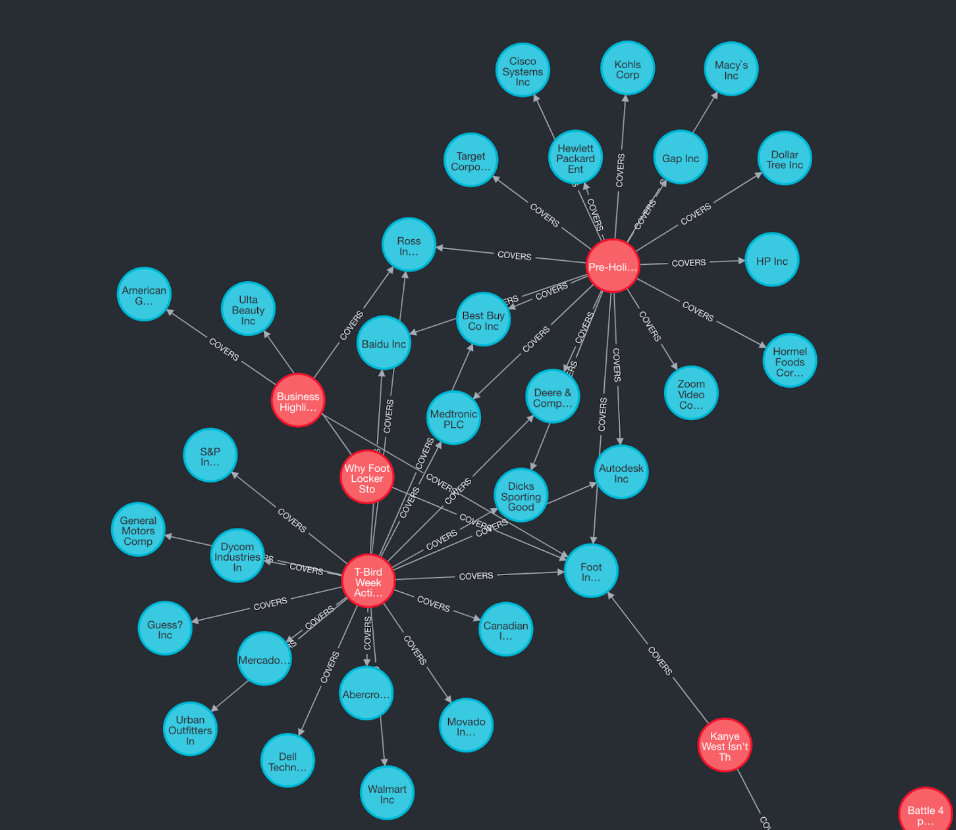
\includegraphics[width=0.8\textwidth]{images/virtual-relationship-between-nodes.png}
 \caption{Virtual relationship between nodes }
 \label{fig:virtual-relationship-nodes}
\end{figure}


\noindent In tables \ref{table:graph-model-properties} and \ref{table:model-properties-relationships} we see our property graph model and the relationships within:

\begin{table}[h]
\centering{
\begin{tabular}{|l|l|l|}
\hline
\textbf{Node}     & \textbf{Relationship} & \textbf{Node}            \\ \hline
NewsItem & COVERS       & Company         \\ \hline
NewsItem & HAS          & TickerSentiment \\ \hline
NewsItem & HAS          & Topic           \\ \hline
Company  & IS\_IN       & Sector          \\ \hline
Company  & HAS          & Price           \\ \hline
\end{tabular}%
}
\caption{Graph model properties }
\label{table:graph-model-properties}
\end{table}

\begin{table}[h]
\centering{
\begin{tabular}{|l|l|l|}
\hline
\textbf{Node/Relationship}     & \textbf{Properties}\\ \hline
NewsItem & \begin{tabular}[c]{@{}l@{}} - url \\ - time\_pusblished \\ - summary \\ - overall\_sentiment\_score \\ - overall\_sentiment\_label
\end{tabular} \\ \hline
Company & \begin{tabular}[c]{@{}l@{}} - ticker \\ - name \\ - description \\ - company\_sector\_name \\ 
\end{tabular} \\ \hline
Topic & \begin{tabular}[c]{@{}l@{}} - topic \\ - relevance\_score \end{tabular} \\ \hline
Sector  & \begin{tabular}[c]{@{}l@{}} - sector\_name  
\end{tabular} \\ \hline
Price  & \begin{tabular}[c]{@{}l@{}} - company\_ticker \\ - date \\ - open \\ - close \\ 
\end{tabular} \\ \hline
\end{tabular}%
}
\caption{Model properties relationships }
\label{table:model-properties-relationships}
\end{table}

\noindent Overall, such a property graph model, saved in Neo4j, allows us to perform necessary queries to analyse the news coverage of the stock market.

\noindent Figure \ref{fig:virtual-relationship-nodes} shows the visualisation of the relationship between nodes NewsItem (red colour) and Company (blue colour).\\
\\
\noindent Figure \ref{fig:virtual-relationship-nodes-sectors} shows the visualisation of the virtual relationship between nodes NewsItem (red colour) and Sector (orange colour). \\
\\
While NewsItem does not have a direct relationship to Sector, we can create a virtual one (called ``COVERS\_INDUSTRY``) while performing a search query. It is done without changing our underlying graph model. 
\\
That is possible because NewsItem has a direct relationship to Company, and Company has a direct relationship to Sector.

\begin{figure}[h]
 \centering
 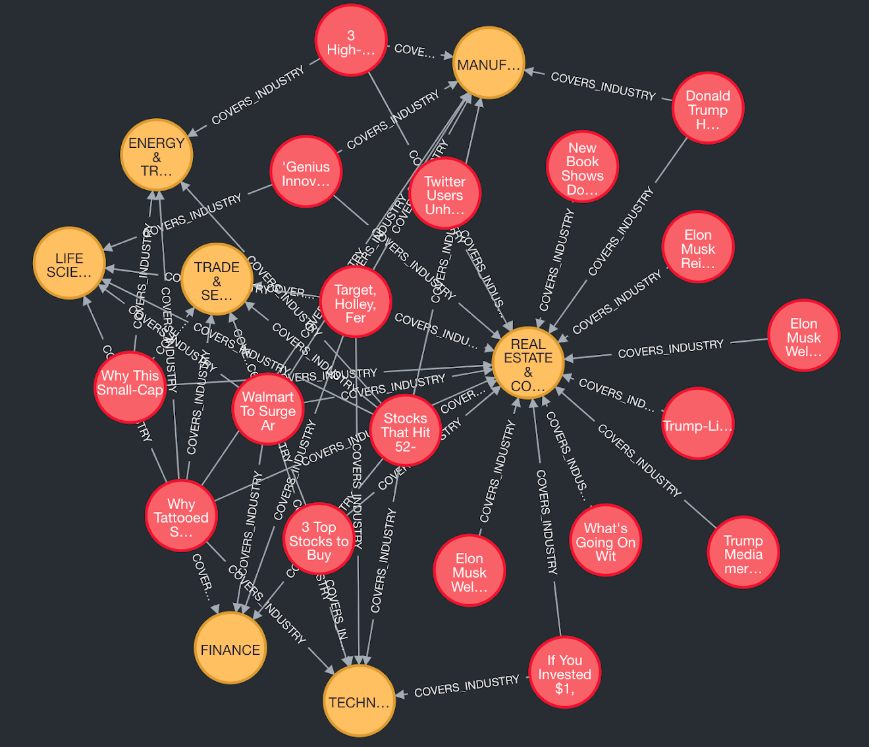
\includegraphics[width=0.8\textwidth]{images/virtual-relationship-between-nodes-sectors.png}
 \caption{Virtual relationship between nodes and sectors }
 \label{fig:virtual-relationship-nodes-sectors}
\end{figure}

\newpage

\noindent To create such a model from the data we gathered, we had to write several algorithms, as well as our own database parser. Here is a short explanation of the implementation part:

\begin{itemize}
\item[-] we perform breadth-first-search, where the first node is a randomly selected company;
\item[-] we request the news for a certain range for this company (one month); 
\item[-] if the news article was visited before, we ignore it;
\item[-] we save news article, its topic, sentiment for every company mentioned, as well as each company itself, in the database;
\item[-] We gather the following information for every company mentioned: what industry sector the company is, as well as one month of stock price data in the month the news article was published;
\item[-] if the company is encountered again, we request the news starting from the previous earliest date
\end{itemize}
\chapter{Interpretation}
\label{cha:interpretation}

\section{Hypothesis 1}
\label{cha:hypothesis-1}
\subsection{The media covers securities based on their industry sector}

Financial instruments, such as stocks and bonds, are frequently classified into market sectors to enable comparison of companies with similar operations. Each sector possesses unique traits and considerations that can affect the desirability of investments within that sector. An investment manager may opt to concentrate on a particular sector or diversify by including various sectors in their portfolio.
Market sectors provide a valuable structure for assessing potential investments and identifying which securities may be most pertinent to monitor within a specific sector. This can be especially useful when building a portfolio with a predetermined market weighting. By considering the specific characteristics of different sectors, an investor can make more informed decisions about which investments to include in their portfolio. \cite{kalyani2016stock}

The media plays a significant role in shaping public perception and understanding of various industries and companies. In particular, the media often covers securities, or financial instruments such as stocks and bonds, based on the industry sector to which they belong. This coverage can have a significant impact on the perceived value and performance of these securities. For example, a company that operates in a rapidly growing industry may receive more media attention and be seen as a more attractive investment opportunity compared to a company in a slower-growing industry \cite{MediaCov52:online}. Similarly, negative media coverage of a particular industry sector may lead to negative perceptions and lower demand for securities within that sector. Understanding the media's coverage of securities based on their industry sector can therefore be important for investors seeking to make informed investment decisions.

It is proven by different papers that news sentiments can have an impact on the behavior of stock charts. This is because news articles, particularly those related to a company's financial performance, can contain valuable information about the company's future prospects and thus influence its stock price. In the research “Stock trend prediction using news sentiment analysis” \cite{kalyani2016stock} the authors used non-quantitative data, specifically financial news articles about a company, to predict the future trend of its stock. Main goal of the research was to examine the relationship between news and stock trends by classifying the polarity of the news articles as positive or negative. Three different classification models were created with subsequent evaluation of their performance. The results showed that the Random Forest and Support Vector Machine models performed well, while the Naive Bayes model had slightly lower performance. Overall, the accuracy of the prediction model was found to be more than 80\%, which represents an improvement of 30\% compared to random labeling of news articles with 50\% accuracy \cite{kalyani2016stock}. 
Another group conducted a research and analyzed news sentiments related to the stock market, and developed a sentiment analysis dictionary which had a directional accuracy of about 70\%.The authors also mention that previous research has demonstrated that various forms of online information, such as Wikipedia usage patterns, news stories, and social media consumption, can affect investors' opinions and subsequently, financial markets \cite{1812041948:online}

\newpage
In this paper, we use a graph database to firstly focus on the hypothesis if the media coverage of securities also propagates to other stocks in the same industry sector, without considering the price, but rather examining other equities within the same industry sector.  For instance, it is of interest to examine whether media sources tend to report on securities from the same industry sector following coverage by a single media source, or if the coverage is limited to the specific security initially reported on.


\noindent To prove or disprove the first hypothesis, we explore the graph data, gathered as described in chapter \ref{cha:methodology}.\\
First, we need to get all the NewsItems from the gathered data. According to the specifics, described in the chapter \ref{cha:model}, the NewsItems have the following relationships and properties, as seen in the following example of news coverage for the company Lockheed Martin:

\begin{lstlisting}[caption={Example properties of a NewsItem}, captionpos=b, label={lst:example-properties-newsitem}]
"properties": {
    "summary": "Lockheed (LMT) reported earnings 30 days ago. What's next for the stock? We take a look at earnings estimates for some clues.",
    "source_domain": "www.zacks.com",
    "overall_sentiment_label": "Somewhat-Bullish",
    "category_within_source": "n/a",
    "overall_sentiment_score": 0.19736,
    "source": "Zacks Commentary",
    "banner_image": "https://staticx-tuner.zacks.com/images/default_article
                    _images/default70.jpg",
    "title": "Lockheed  ( LMT )  Up 6% Since Last Earnings Report: Can It Continue?",
    "time_published": "2022-11-17T16:30:18",
    "url": "https://www.zacks.com/stock/news/2019526/lockheed-lmt-up-6-since-last
            -earnings-report-can-it-continue",
    "authors": [
      "Zacks Investment Research"
    ]
  },
}
\end{lstlisting}

Following query can be used to get all the NewsItems:

\begin{lstlisting}[caption=Get all NewsItem Cypher Query, captionpos=b, language=bash, label={lst:getall-newsitem-cypher}]
MATCH (n:NewsItem) RETURN n LIMIT 1000
\end{lstlisting}

\noindent This yields the following graph:

\begin{figure}[h]
 \centering
 \includegraphics[width=0.5\textwidth]{images/newsItemsAll.png}
 \caption{Raw data with 546 NewsItem nodes }
 \label{fig:raw-data-546-newsitem-nodes}
\end{figure}

It is important to consider that NewsItems have a relationship of ``COVERS`` to a specific Company and ``HAS`` to TickerSentiment and Topic. This data can then be synthesized to establish a new relationship between NewsItems and Sectors.

\noindent Query from Listing \ref{lst:relationship-newsitems-sectors} can be used for that:

\begin{lstlisting}[caption={Relationship between NewsItems and Sectors},label={lst:relationship-newsitems-sectors},captionpos=b]
MATCH (n:NewsItem)-[:COVERS]-(c:Company)-[:IS_IN]-(s:Sector)
WITH n, collect(distinct s) as ns
UNWIND ns as N
CALL apoc.create.vRelationship(n,'COVERS_INDUSTRY',{}, N) YIELD rel
RETURN n, rel, N
\end{lstlisting}

\noindent This yields the following graph with 503 NewsItems and 7 Sectors

\begin{figure}[h]
 \centering
 \includegraphics[width=0.7\textwidth]{images/newsItemCoverageSector.png}
 \caption{NewsItems and their Sector coverage }
 \label{fig:newsitems-sector-coverage}
\end{figure}

In this example, we will investigate the relationship between news coverage and the behavior of Apple stock, considering the time factor. To do this, we will collect data on news articles related to the stock over a specific period of time and analyze the volume and tone of the coverage. 
The time factor is an important consideration when studying the relationship between news coverage and stock behavior, as it can provide insights into the public perception and understanding of the company and its performance. By examining the news coverage and stock behavior over a specific period of time, we can better understand the impact of the media on financial markets. In addition to examining the time factor, it is also important to consider other factors that may impact the stock's behavior, such as market conditions, economic indicators, and news events related to the company or industry. \cite{2107087294:online}

\newpage
\noindent The following query (Listing: \ref{lst:relationship-apple-time}) allows the retrieval of NewsItems that covered Apple within the time frame of October to November 2022, each beginning of the month:\\

\begin{lstlisting}[caption={Relationship of NewsItems to Apple Stock october till november}, label={lst:relationship-apple-time},captionpos=b]
MATCH (n:NewsItem)-[:COVERS]-(c:Company{name:"Apple Inc"})-[:IS_IN]-(s:Sector{sector_name:"TECHNOLOGY"})
WITH n, collect(distinct s) as ns
UNWIND ns as N
CALL apoc.create.vRelationship(n,'COVERS_INDUSTRY',{}, N) YIELD rel
WHERE datetime(n.time_published) >= datetime("2022-10-01T00:00:00") AND datetime(n.time_published) < datetime( "2022-11-01T00:00:00")
RETURN n, rel, N
\end{lstlisting}

\noindent This produces a single result, meaning Apple was covered only once, by Motley Fool:

\begin{table}[h]
\centering
\resizebox{\columnwidth}{!}{%
\begin{tabular}{|l|l|}
\hline
Summary                                                                         & overall\_sentiment\_label \\ \hline
Plus a look at investing books, stocks to watch, and other topics for investors & Neutral                   \\ \hline
\end{tabular}%
}
\end{table}

\noindent No notable events occurred until November 8th, when Apple received coverage from Benzinga with the following content in the title: “Apple To \$180? Plus Piper Sandler Predicts \$132 For Take-Two Interactive” Following graph chart (see Fig. \ref{fig:newsitems-apple-coverage-october-8th-november} is the output of the query above, with the timeframe october - 08th november:


\begin{figure}[h]
 \centering
 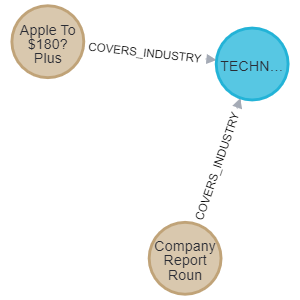
\includegraphics[width=0.3\textwidth]{images/apple-two-news.png}
 \caption{Apple coverage october to 8th of november }
 \label{fig:newsitems-apple-coverage-october-8th-november}
\end{figure}

The news article from Benzinga mentions Apple in the context of a decline in its share price, which is reportedly linked to an event involving Take-Two-Interactive. To further investigate this, we will analyze the coverage of Apple stock in the Technology sector from November 08th to November 30th (a period of twenty two days). The query remains same with only modification to the end date:

\begin{lstlisting}[caption={Datetime modification for the query in Listing \ref{lst:relationship-apple-time}}\label{lst:query-mod-rel-apple-time},captionpos=b]
< datetime( "2022-11-30T00:00:00")
\end{lstlisting}

After implementing this modification, we see that the coverage of Apple and the Technology sector significantly increased, resulting in the identification of 20 NewsItems that mention Apple. This increase in coverage could be due to a variety of factors, such as an increase in media interest in the company after the initial Apple coverage by Benzinga.

\begin{figure}[h]
 \centering
 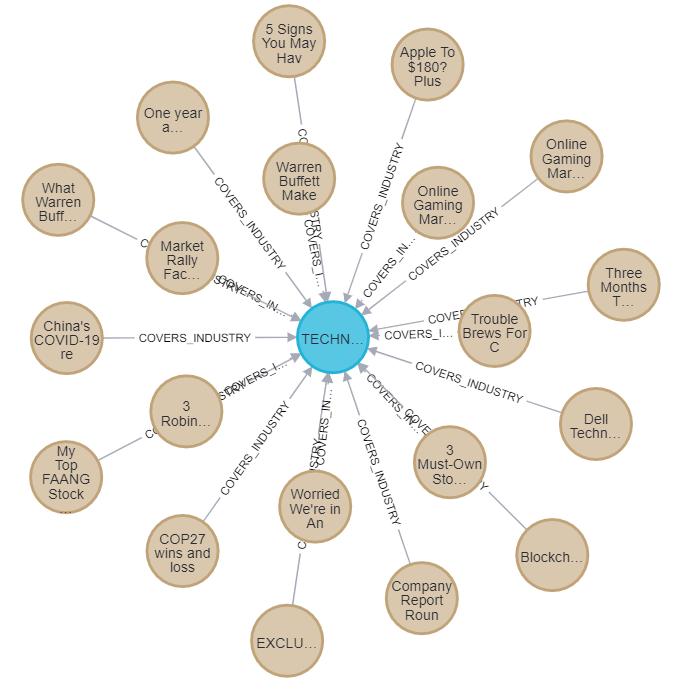
\includegraphics[width=0.5\textwidth]{images/apple-after-benzinga.png}
 \caption{Apple stock after Benzinga news coverage }
 \label{fig:newsitems-apple-after-benzinga-coverage}
\end{figure}

Upon analyzing the overall\_sentiment\_label property of the NewsItems that cover Apple in the time frame described above, 8 of them had a somewhat-bullish sentiment, 1 had a somewhat-bearish sentiment, and 11 had a neutral sentiment. This distribution of sentiments suggests that the news coverage of Apple was relatively positive, with a slightly higher proportion of neutral articles. \\
\\
To further investigate this topic, we examined the coverage of Take-Two Interactive Software from the beginning of October to the 8th of November, which did not yield any coverage from news providers. After the publication of the article about Apple stock in relation to Take-Two-Interactive on November 8th, we compared the coverage from November 9th to the 30th and found 17 NewsItems covering the company. This analysis provides further evidence of the influence of media coverage on the behavior of stocks, as the publication of the article about Apple appeared to spark an increase in coverage of Take-Two Interactive.\\
\\
The data in the provided graph database clearly indicates that media coverage tends to be drawn to stocks that receive attention from other NewsItems and is generally focused within the covered sector. This suggests that news articles about certain stocks may be more likely to be published or shared if they are already receiving significant attention from other sources. This phenomenon can provide valuable insights for investors and market analysts, as it can provide an indication of the public perception and behavior of different stocks.



\newpage
\section{Hypothesis 2}
\label{cha:hypothesis-2}
There is a correlation between news sentiment and stock price performance
\subsection{Related work}
As already noted in the chapter \ref{cha:hypothesis-1}
existing studies in sentiment analysis have found that positive news sentiment is associated with positive stock price performance, while negative news sentiment is associated with negative stock price performance. However, the relationship between news sentiment and stock price performance is complex and may depend on various factors, such as the specific company being analyzed and the overall market conditions.\cite{kalyani2016stock}
\subsection{Data analysis}
As a starting point, we continue to look at NewsItems dedicated to Apple Inc, but in combination with the TikerSantiment of NewsItems relating only to that company. 
\begin{lstlisting}[caption={Relationship of NewsItems to Apple Stock with TikerSantiment}, label={lst:newsItems_tikerSantiment_apple},captionpos=b]
MATCH (c:Company {name:"Apple Inc"})-[:HAS]->(p:Price {company_ticker:"AAPL"})
MATCH (n:NewsItem)-[:HAS]->(t:TickerSentiment{ticker:"AAPL"})
MATCH (n:NewsItem)-[:COVERS]->(c{name:"Apple Inc"})
RETURN c,n,t
ORDER BY n.date ASC
\end{lstlisting}

The result of a subsequent query, represented in the graph:
\begin{figure}[h]
 \centering
 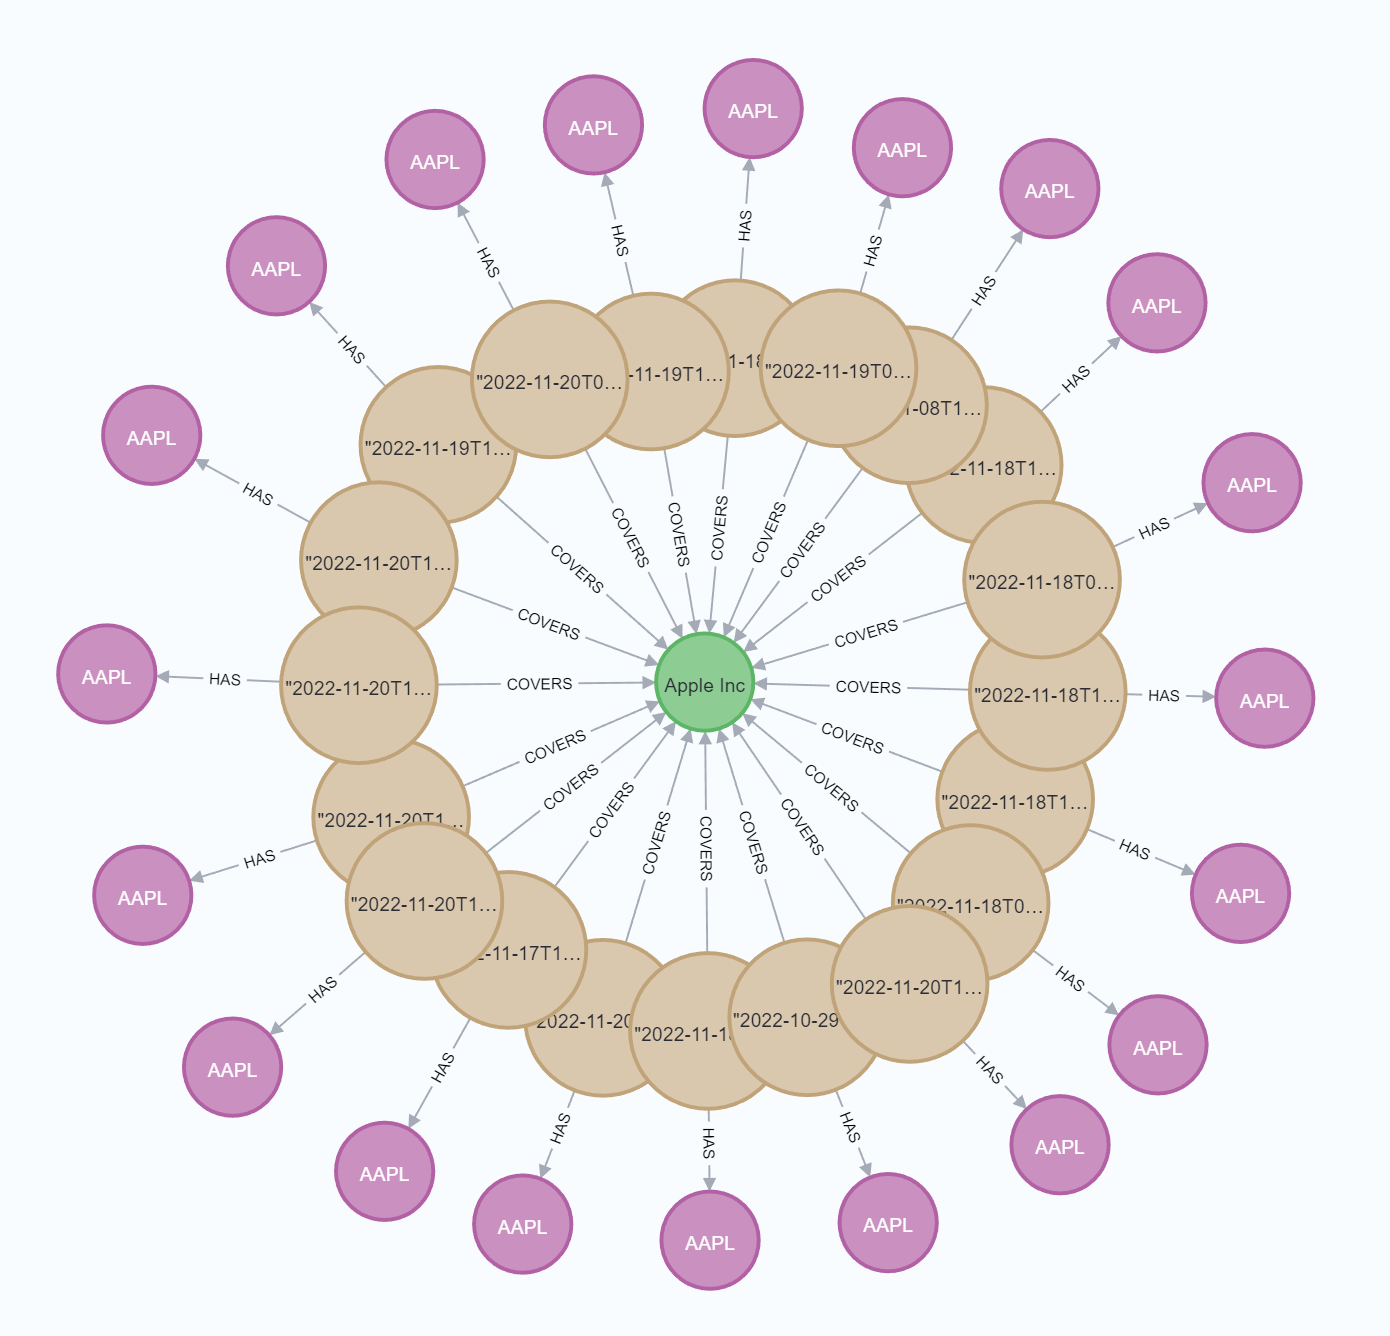
\includegraphics[width=0.6\textwidth]{images/apple_news_ticker_sentiment_graph.png}
 \caption{Relationship of NewsItems to Apple with TikerSantiment }
 \label{fig:apple_news_ticker_sentiment_graph}
\end{figure}

Next, we took a closer look at the development of prices compared to the TickesSentiment of the NewsItem.
\begin{lstlisting}[caption={Relationship of NewsItem TikerSantiment and Price of Apple Stock }, label={lst:newsItems_tikerSantiment_and_price_apple},captionpos=b]
// Appl Inc
MATCH (c:Company {name:"Apple Inc"})-[:HAS]->(p:Price {company_ticker:"AAPL"})
MATCH (n:NewsItem)-[:HAS]->(t:TickerSentiment{ticker:"AAPL"})
MATCH (n:NewsItem)-[:COVERS]->(c{name:"Apple Inc"})
RETURN c.name AS company, p.close AS price, n.time_published AS news_date, p.date AS price_date,  n.overall_sentiment_score AS news_sentiment, t.ticker_sentiment_score AS ticker_sentiment
ORDER BY p.date ASC
\end{lstlisting}

\begin{figure}[h]
 \centering
 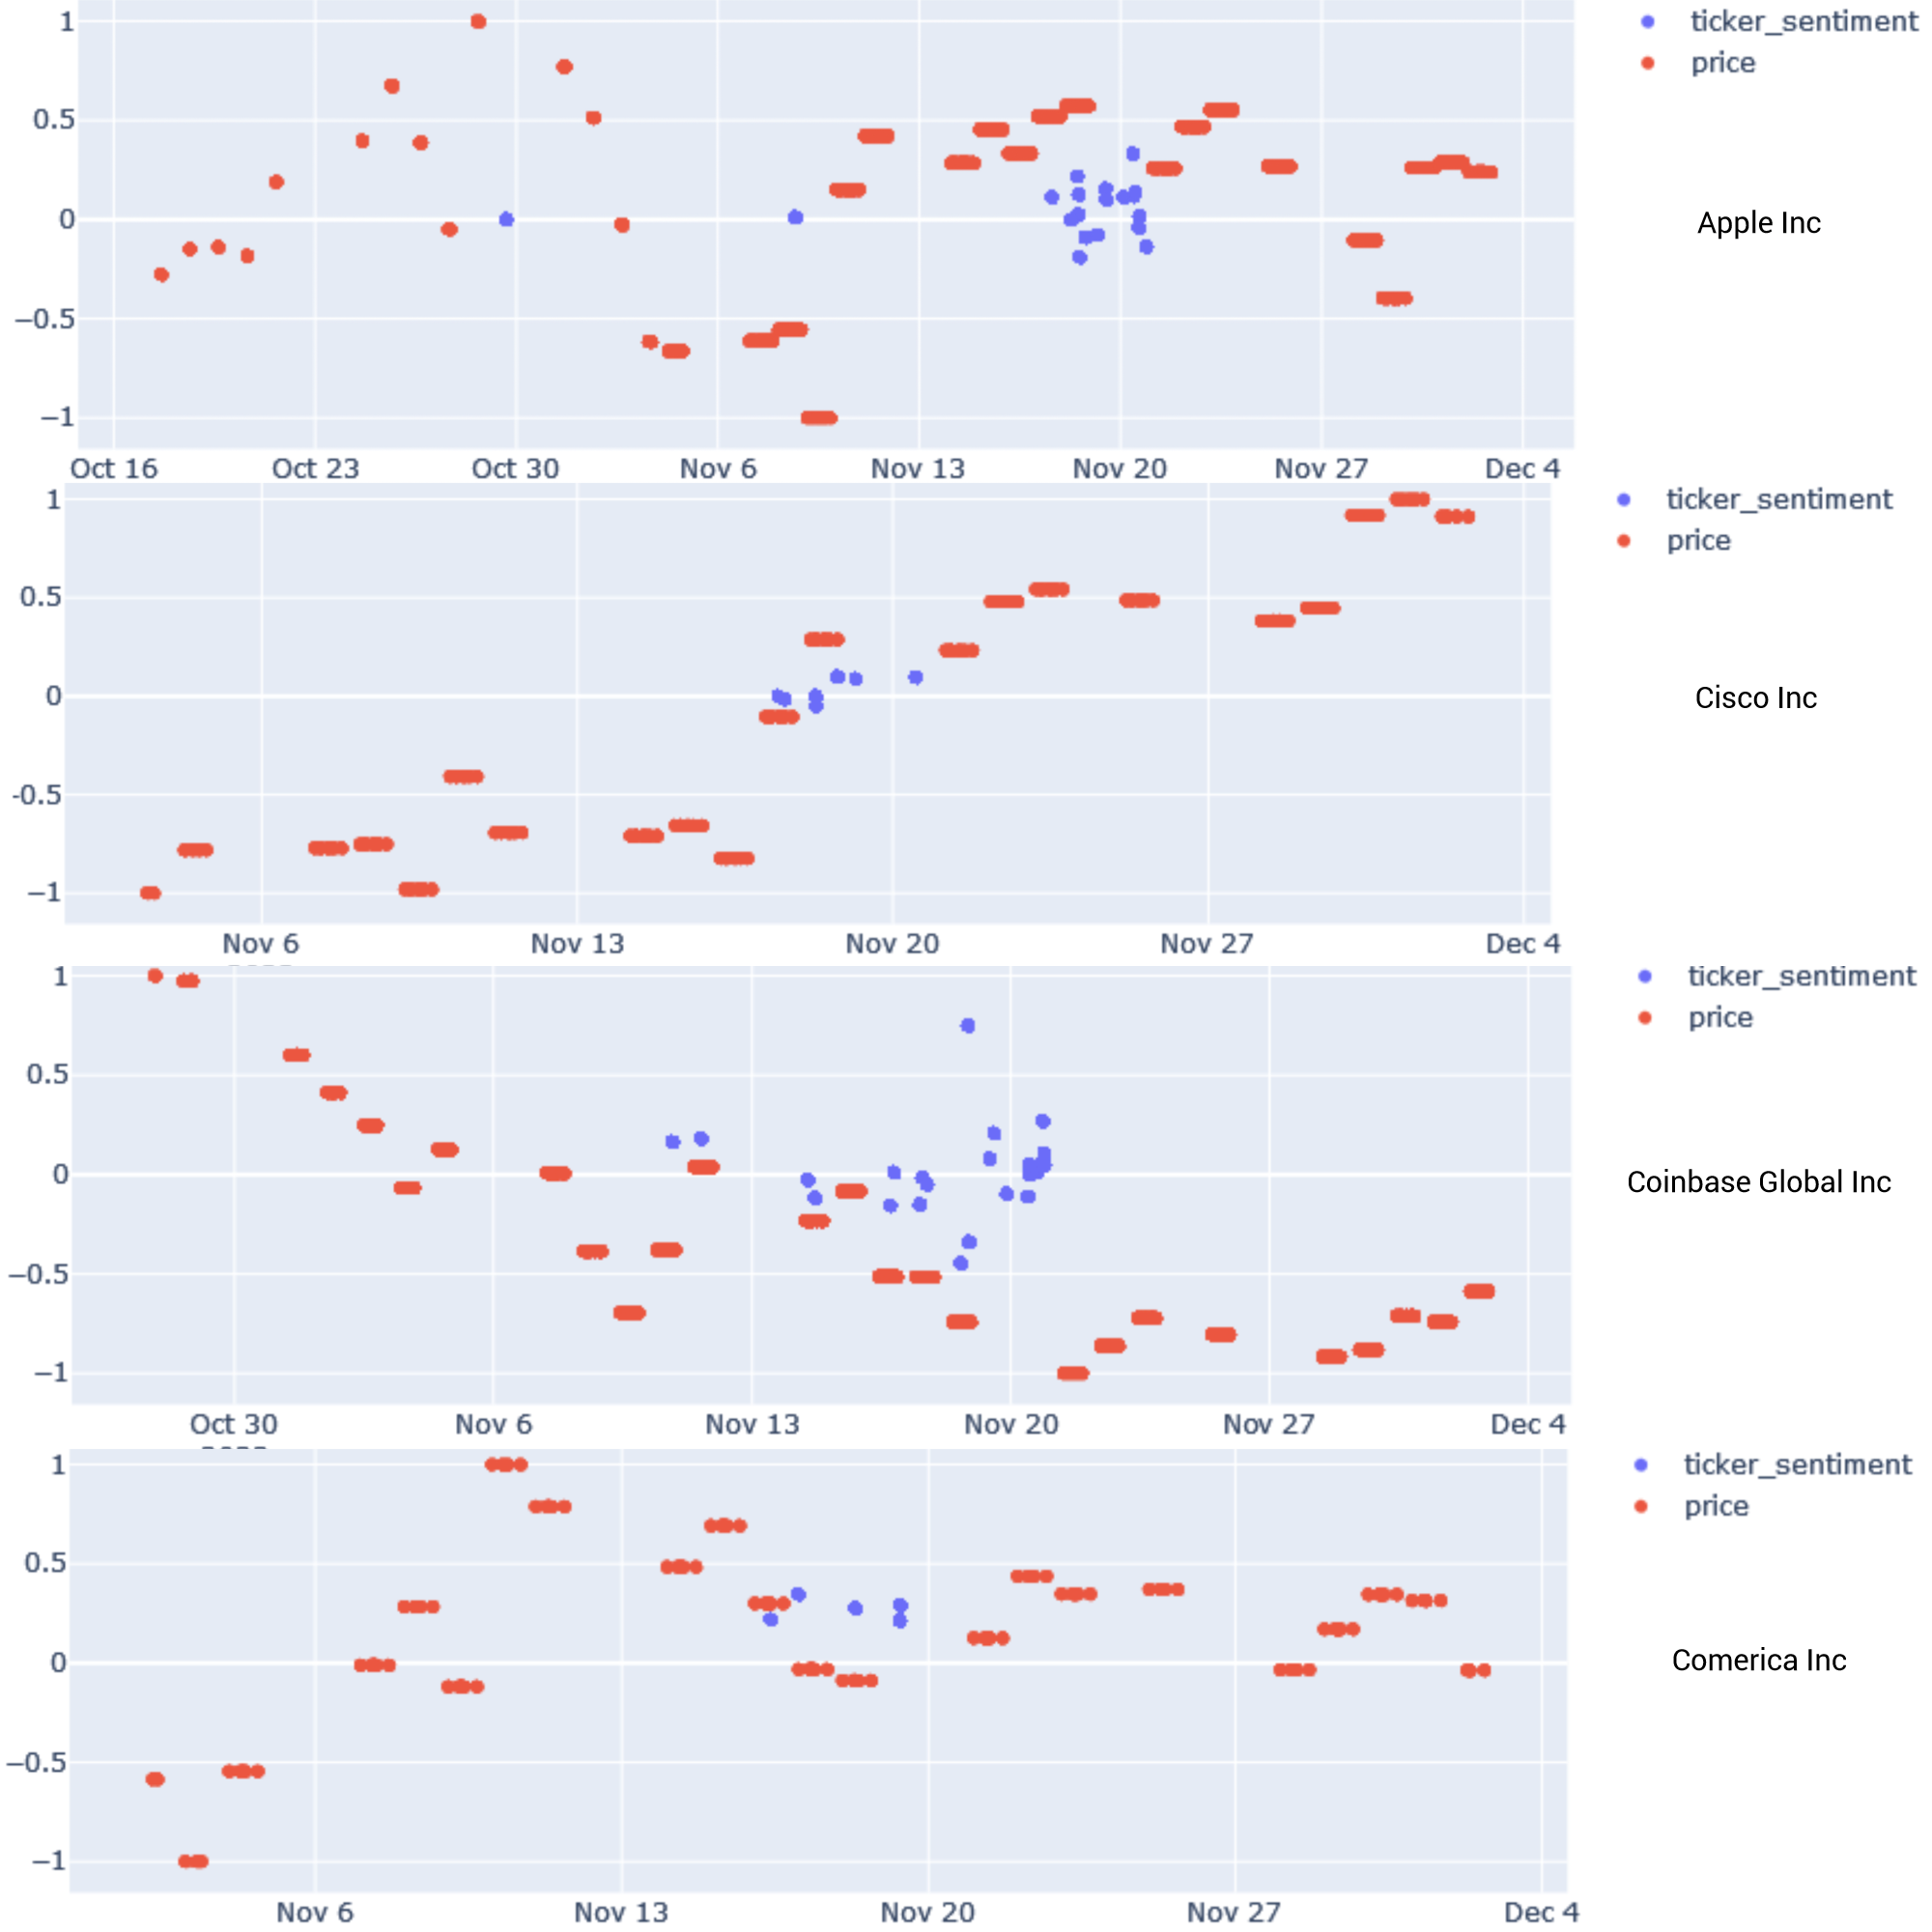
\includegraphics[width=1.0\textwidth]{images/price_news_ticker_charts.png}
 \caption{News TikerSentiment and Price}
 \label{fig:price_news_sentiment}
\end{figure}

This plot shows the relationship between news sentiment and stock price performance for 4 companys over a period of time. The x-axis represents the date, and the y-axis represents the stock price. The red dots showing the stock price over time normalized from -1 to 1, while the blue dots showing the news sentiment on a scale from -1 (extremely negative) to 1 (extremely positive). The plot shows that not always when news sentiment is positive, the stock price tends to increase, and  not always when news sentiment is negative, the stock price tends to decrease.


---

% This plot shows the relationship between news sentiment and stock price performance for a specific industry over a period of time. The x-axis represents the date, and the y-axis represents the average stock price for the industry. The line chart shows the average stock price over time, while the bar chart shows the average news sentiment on a scale from -1 (extremely negative) to 1 (extremely positive). The plot shows that when news sentiment is positive, the average stock price tends to increase, and when news sentiment is negative, the average stock price tends to decrease.
\chapter{Results}
\label{cha:results}
\appendix
\input{appendix/apA} % Appendix A
\backmatter
\bibliographystyle{gerplain}
\bibliography{thesis}
\end{document}

